\chapter{Environments}
\label{app:environments}

\section{Known Environments with Varied Clutter}
Each of the following environments have a dimension of [20, 10]. 
\begin{figure}[H]
    \centering
    \makebox[\textwidth]{
    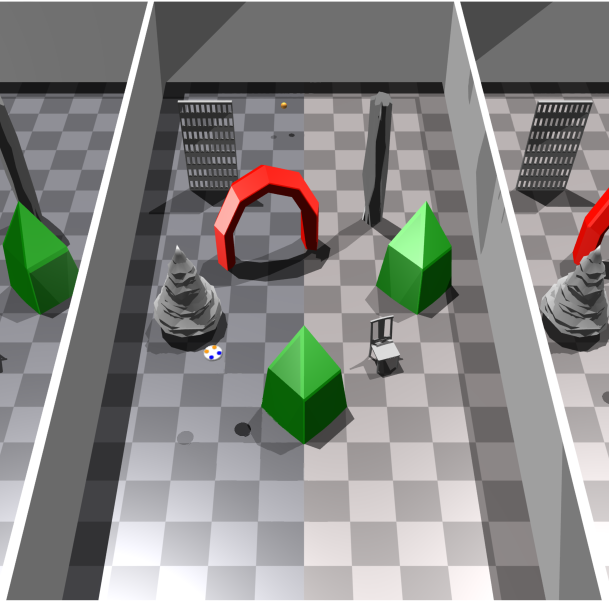
\includegraphics[scale=0.45]{figures/app_envs/easy_flat.png}
    }
    \caption{The easy environment, with 7 obstacles.}
    \label{fig:easy_flat}
\end{figure}
\begin{figure}[H]
    \centering
    \makebox[\textwidth]{
    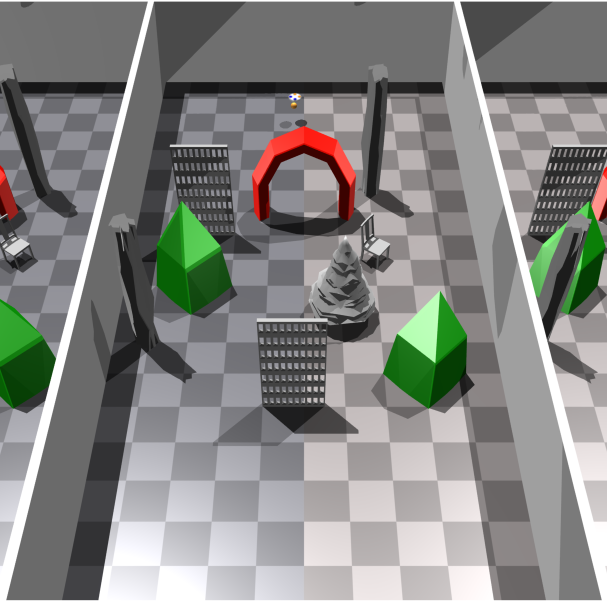
\includegraphics[scale=0.45]{figures/app_envs/medium_flat.png}
    }
    \caption{The medium environment, with 9 obstacles.}
    \label{fig:medium_flat}
    \makebox[\textwidth]{
    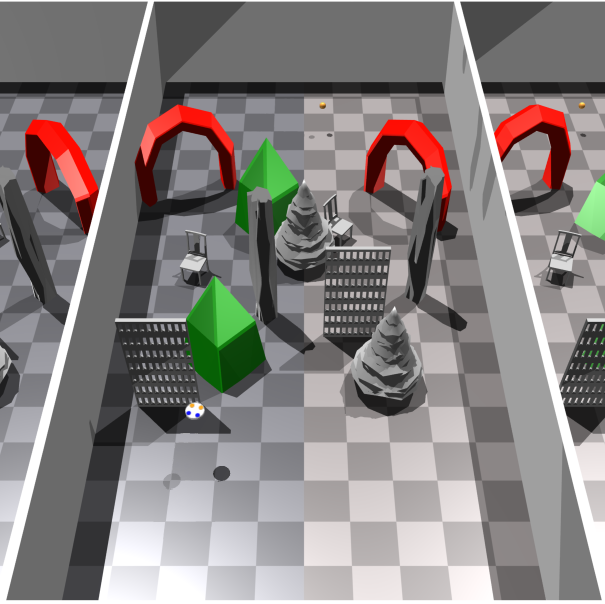
\includegraphics[scale=0.45]{figures/app_envs/hard_flat.png}
    }
    \caption{The hard environment, with 12 obstacles.}
    \label{fig:hard_flat}
\end{figure}
\begin{figure}[H]
    \centering
    \makebox[\textwidth]{
    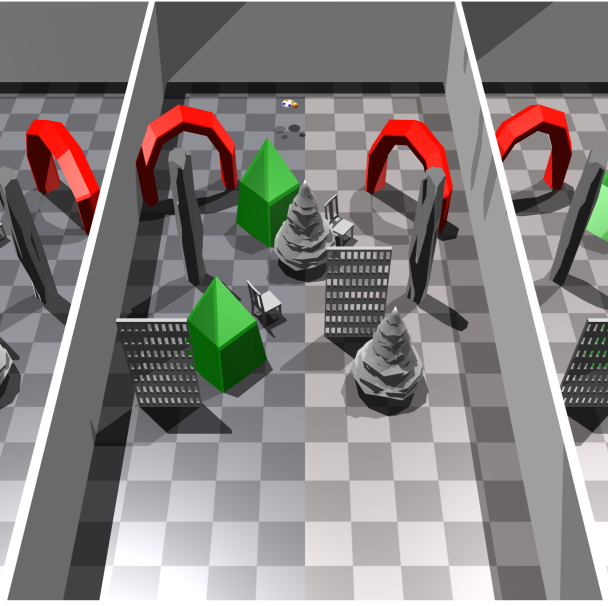
\includegraphics[scale=0.35]{figures/app_envs/hard_swapped_flat.png}
    }
    \caption{The hard-swapped environment, with 12 obstacles. The chair and simple stone in the center are swapped to not artificially block the agent.}
    \label{fig:hard_swapped_flat}
\end{figure}

\section{Large Environment}
\begin{figure}[H]
    \centering
    \makebox[\textwidth]{
    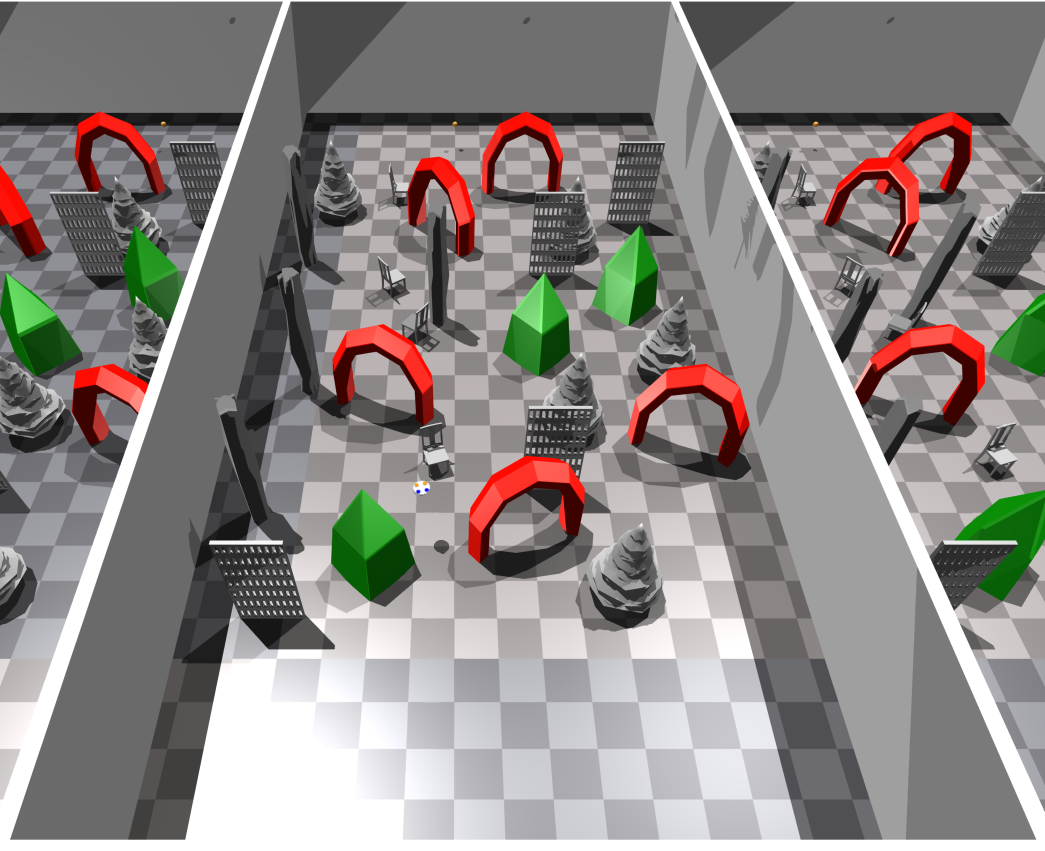
\includegraphics[scale=0.3]{figures/app_envs/large_flat.png}
    }
    \caption{The large environment, with a dimension of [30, 15] and 25 obstacles.}
    \label{fig:large_flat}
\end{figure}